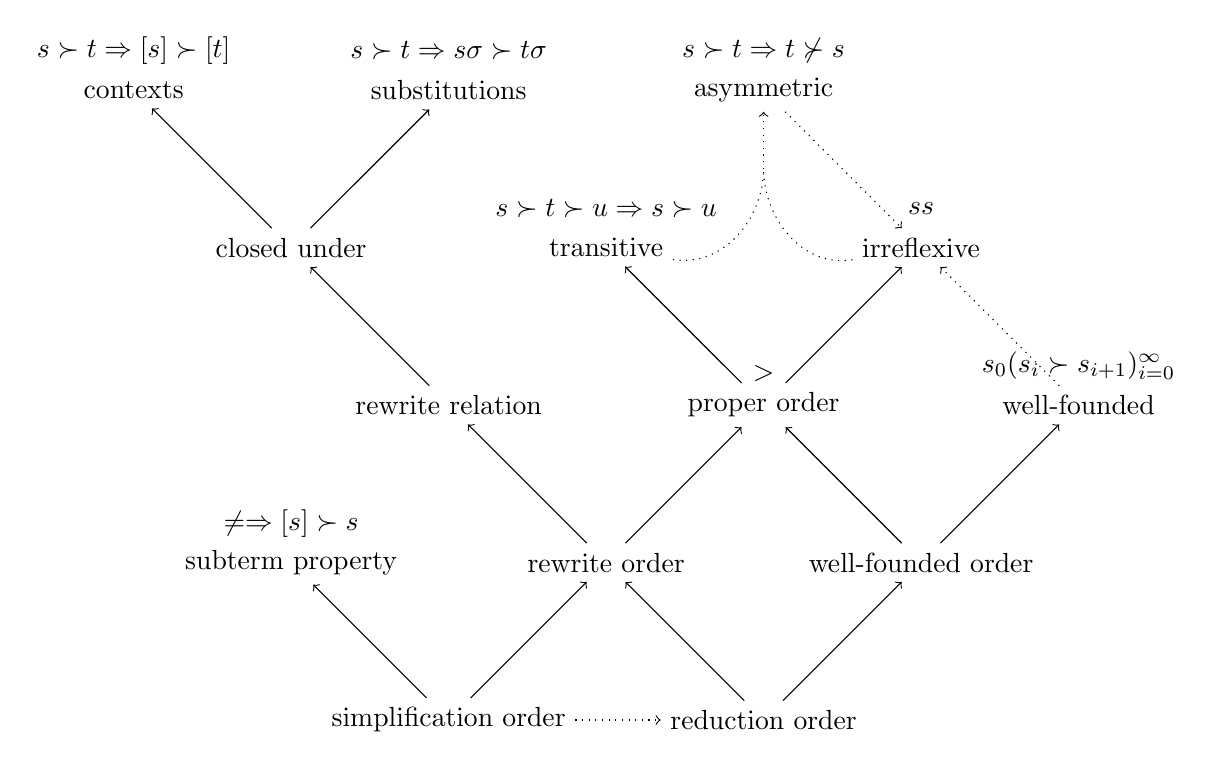
\begin{tikzpicture}
    \node (defCUC) at (-4,8.5) { $s\succ t\Rightarrow \ctx[s]\succ \ctx[t]$};
    \node (CUC) at (-4,8) { contexts };
    \node (defCUS) at (0,8.5) { $s\succ t\Rightarrow s\sigma\succ t\sigma$};
    \node (CUS) at (0,8) { substitutions };

    \node (ASYM) at (4,8.5) { $s\succ t\Rightarrow t\not\succ s$ };
    \node (ASYM) at (4,8) { asymmetric };

        \node (CL) at (-2,6) { closed under };
        \node (defIRR) at (2,6.5) { $s\succ t\succ u\Rightarrow s\succ u$ };
        \node (IRR) at (6,6) { irreflexive };
        \node (defIRR) at (6,6.5) { $s\nsucc s$ };
        \node (TRA) at (2,6) { transitive };

        \node (PO) at (4,4.4) { $>$ };
        \node (PO) at (4,4) { proper order };
        \node (RWR) at (0,4) { rewrite relation };

        \node (defSTP) at (-2,2.5) { $\ctx\neq\ctxhole\Rightarrow \ctx[s]\succ s$ };
        \node (STP) at (-2,2) { subterm property };
        \node (RWO) at (2,2) { rewrite order };
        \node (defWF) at (8,4.5) { $\nexists s_0(s_i\succ s_{i+1})_{i=0}^{\infty}$ };
        \node (WF) at (8,4) { well-founded };

        \node (SO) at (0,0) {simplification order};
        \node (RO) at (4,0) {reduction order};

        \node (WFO) at (6,2) { well-founded order };


        \draw[->] (CL) -- (CUC);
        \draw[->] (CL) -- (CUS);

        \draw[->] (PO) -- (IRR);
        \draw[->] (PO) -- (TRA);

        \draw[->] (RWR) -- (CL);

        \draw[->] (RWO) -- (PO);
        \draw[->] (RWO) -- (RWR);

        \draw[->] (SO) -- (STP);
        \draw[->] (RO) -- (RWO);
        \draw[->] (RO) -- (WFO);
        % \draw (RO) edge[out=0,in=-45,->] (WF);

        \draw[->] (SO) -- (RWO);
        \draw[->, dotted] (SO) -- (RO);

        \draw[->] (WFO) -- (WF);
        \draw[->] (WFO) -- (PO);

        \draw[->, dotted] (WF) -- (IRR);

        % \node (TRAIRR) at (4,7) { $\bullet$ };
        \draw[->, dotted] (4,7) -- (ASYM);

        \draw[dotted] (TRA) edge [out=-10, in=-90] (4,7);
        \draw[dotted] (IRR) edge [out=190, in=-90] (4,7);

        \draw[->, dotted] (ASYM) -- (IRR);
        % \draw[->, dotted] (ASYM) edge [out=0, in=0] (IRR);


    \end{tikzpicture}